\subsection{Structural Responses to Bounded Relaxation}
  \label{subsec:structural-interpretation-projective-thermodynamics}

  Physical observables arise through a generically non-injective projection
  $\Pi : \Omega \rightarrow O$ from the relational substrate $\Omega$.
  The $\chi$ substrate evolves under a bounded relaxation flux,
  characterized by a Born--Infeld-type constraint $b_{\mathrm{BI}}$.
  This bound limits the admissible transfer of relational relaxation
  and prevents divergence of effective observables.

  When the relaxation flux approaches its admissible bound,
  the projection enters a saturation regime.
  In such regimes, distinct underlying configurations
  become structurally indistinguishable at the level of $O$.
  This loss of distinguishability induces an objective structural entropy
  associated with the projection:
  \begin{equation}
    S_{\Pi} = -\sum_{o \in O}
    \mu(\Pi^{-1}(o)) \log \mu(\Pi^{-1}(o)),
  \end{equation}
  which reflects non-injectivity rather than epistemic uncertainty.

  \paragraph{Dual structural responses to bounded relaxation.}

    When the relaxation flux approaches its admissible bound,
    the projection $\Pi$ enters a saturation regime.
    Distinct underlying configurations become structurally identified,
    and the effective description must compensate.

    Two structurally distinct responses may occur,
    depending on whether collective reorganization of the projected fiber
    is dynamically accessible.

    \medskip
    \textbf{(A) Thermodynamic compensation: projection-limited heating.}

    In incoherent or weakly correlated systems,
    collective stabilization of the fiber is not available.
    The unresolved relational flux is therefore absorbed into
    effective thermodynamic descriptors.
    Temperature acts as a Lagrange multiplier compressing
    unresolved relational structure into the observable sector.

    Magnetically guided dilute plasmas,
    such as the solar corona,
    illustrate this regime.
    Reduced projectability under strong magnetic structuring
    leads to an elevated effective temperature,
    interpretable as a compensatory response to bounded relaxation
    rather than as excess local energy density.

    \medskip
    \textbf{(B) Coherent reorganization: projective expulsion.}

    In strongly coherent collective phases,
    the system may instead reorganize its internal fiber structure
    so as to preserve maximal projective stability.
    Rather than inflating thermodynamic variables,
    the projected description modifies its admissible connection structure.

    Superconductivity provides a paradigmatic example.
    Collective phase locking of the $U(1)$ fiber
    suppresses internal fluctuations and enforces
    near-vanishing covariant phase gradients in the bulk.
    The Meissner effect may therefore be interpreted
    as the expulsion of incompatible connection curvature,
    maintaining projective stability within the coherent phase.

    \medskip
    These two regimes represent alternative structural resolutions
    of the same constraint:
    bounded relational relaxation under non-injective projection.

  \paragraph{Unified interpretation.}

    These two responses do not represent distinct physical mechanisms,
    but alternative structural resolutions of the same constraint:
    bounded relational relaxation under non-injective projection.

    Thermodynamic variables, geometric curvature,
    horizon formation, and collective coherence
    all act as compensatory descriptors of unresolved relational structure.
    Which response occurs depends on whether
    collective reorganization of the projected fiber
    is dynamically accessible.

    The bounded character of substratic relaxation ensures that
    projection-induced thermodynamic and geometric quantities remain finite.
    This renders the framework predictive despite
    the intrinsic non-injectivity of $\Pi$.

    \begin{figure}[t]
      \centering
      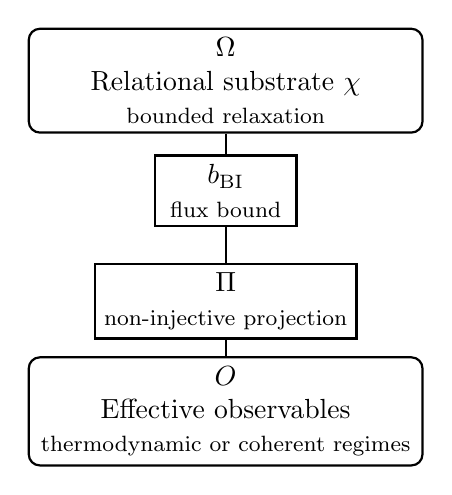
\begin{tikzpicture}[
        node distance=1.4cm,
        every node/.style={align=center},
        box/.style={draw, rounded corners, thick,
        minimum width=5cm, minimum height=1cm},
        narrow/.style={draw, thick,
        minimum width=1.8cm, minimum height=0.8cm}
      ]
    \node[box] (omega)
    {$\Omega$\\Relational substrate $\chi$\\
    {\footnotesize bounded relaxation}};
    \node[narrow, below of=omega] (bi)
    {$b_{\mathrm{BI}}$\\
    {\footnotesize flux bound}};
    \node[narrow, below of=bi] (pi)
    {$\Pi$\\
    {\footnotesize non-injective projection}};
    \node[box, below of=pi] (obs)
    {$O$\\Effective observables\\
    {\footnotesize thermodynamic or coherent regimes}};
    \draw[thick] (omega) -- (bi);
    \draw[thick] (bi) -- (pi);
    \draw[thick] (pi) -- (obs);
      \end{tikzpicture}
      \caption{Structural responses to bounded relaxation.
      Approach to the flux bound may induce either compensatory
      thermodynamic descriptors or coherent projective reorganization,
        depending on collective accessibility of the fiber structure.}
      \label{fig:projective-hourglass}
    \end{figure}
